% Image wrapper: PDF table structure was not recoverable automatically.
% Requires \usepackage{graphicx}. Replace the image with tabular cells when editable text is needed.
% Caption: Figure 2 shows an example of embedding neuro-inspired dynamic sparsity in a vision sensor. Retinal circuits respond primarily to chan- ges in the visual field25, and event camera pixels26mimic this behavior byproducingoutputeventsonlywhenbrightnesschangesabovea certain threshold occur. These neuromorphic sensors generate sparse, low-latencyeventstreamsthatbettercapturedynamicvisualinfor- mationwithouttheredundancyofframe-basedinput,offeringsub- stantialadvantageintermsoflatency,temporalresolution,energy efficiency, and dynamic range27. The neural foundation of dynamic sparsityas well as itsdemon- stratedeffectivenessinneuromorphicvisionsensors,motivatethe exploration of its broader applications in energy-efficient AI. To con- nectinsightsfromneurosciencewiththerecentprogressinvarious fields—such as neuromorphic engineering, deep learning, and domain- specificaccelerators—andtosystematicallyframethekeydesign considerationsforimplementingthisprinciple,thenextsectionela- borates a necessary taxonomy of dynamic sparsity.
\begin{tabular}{c}
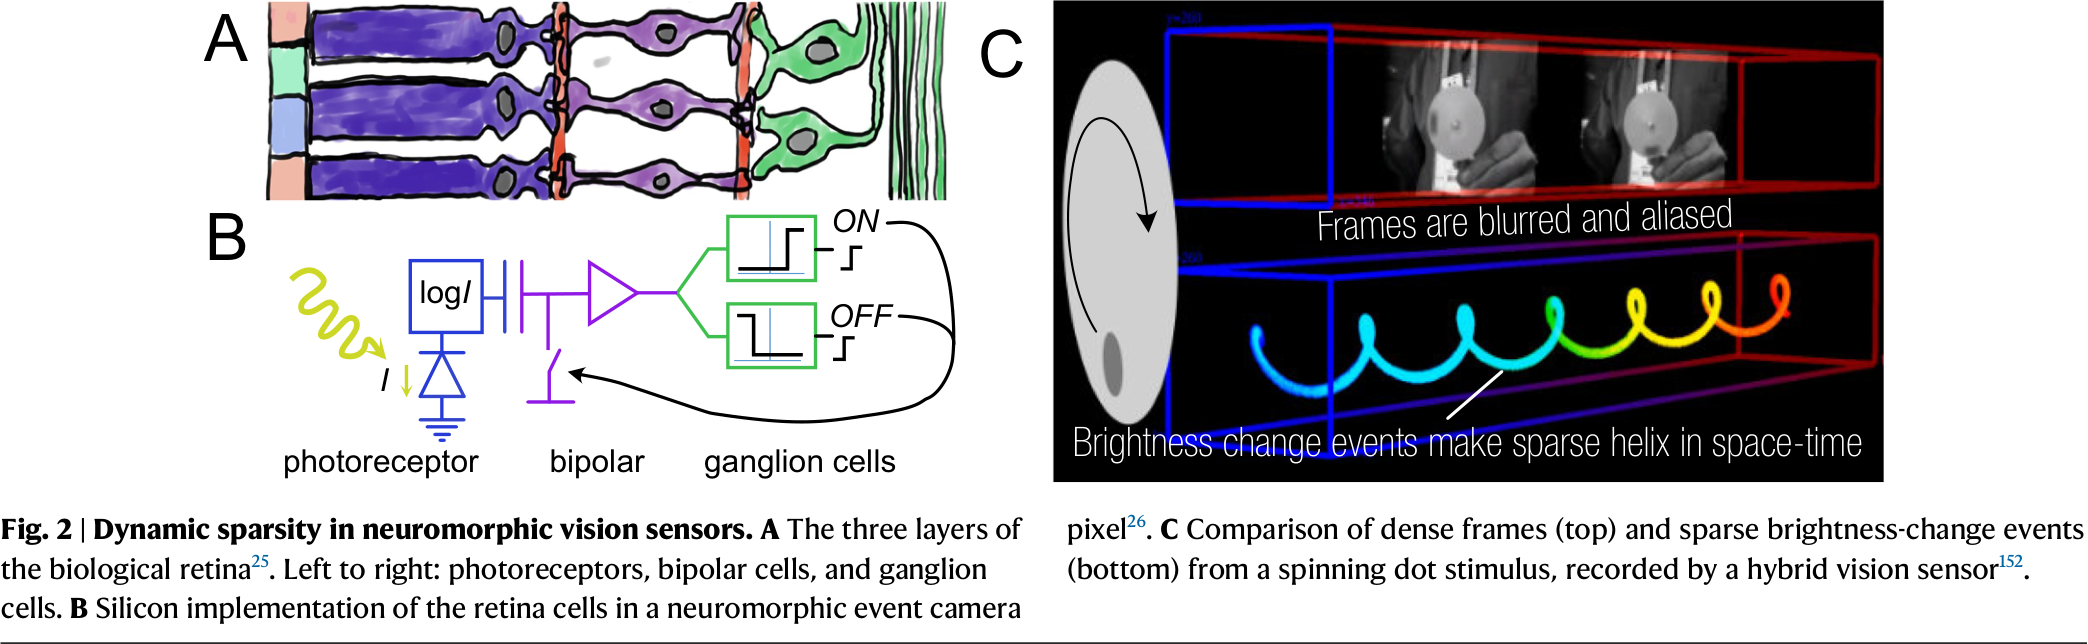
\includegraphics[width=\linewidth]{../original/Table2_p002.png}
\end{tabular}
